\documentclass[tikz,border=4pt]{standalone}
\usepackage{pgfplots}\usepgfplotslibrary{groupplots}
\pgfplotsset{compat=1.18}
\definecolor{corba}{HTML}{365FB3}\definecolor{punt}{HTML}{B91C1C}
\begin{document}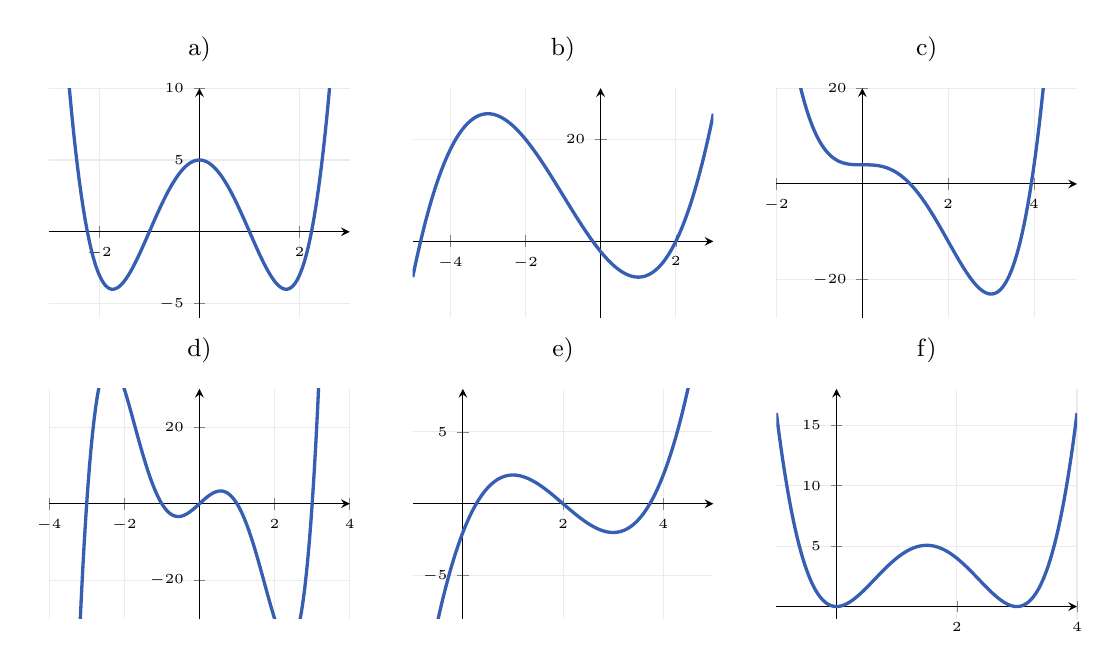
\begin{tikzpicture}
\begin{groupplot}[group style={group size=3 by 2,horizontal sep=0.8cm,vertical sep=0.9cm},
 width=5.4cm,height=4.5cm,axis lines=middle,grid=major,grid style={black!8},tick label style={font=\tiny},title style={font=\small},samples=160]
\nextgroupplot[title={a)},xmin=-3,xmax=3,ymin=-6,ymax=10]\addplot[corba,very thick,domain=-3:3]{x^4-6*x^2+5};
\nextgroupplot[title={b)},xmin=-5,xmax=3,ymin=-15,ymax=30]\addplot[corba,very thick,domain=-5:3]{x^3+3*x^2-9*x-2};
\nextgroupplot[title={c)},xmin=-2,xmax=5,ymin=-28,ymax=20]\addplot[corba,very thick,domain=-2:5]{x^4-4*x^3+4};
\nextgroupplot[title={d)},xmin=-4,xmax=4,ymin=-30,ymax=30]\addplot[corba,very thick,domain=-3.4:3.4]{x^5-10*x^3+9*x};
\nextgroupplot[title={e)},xmin=-1,xmax=5,ymin=-8,ymax=8]\addplot[corba,very thick,domain=-1:5]{(x-2)^3-3*(x-2)};
\nextgroupplot[title={f)},xmin=-1,xmax=4,ymin=-1,ymax=18]\addplot[corba,very thick,domain=-1:4]{x^2*(x-3)^2};
\end{groupplot}\end{tikzpicture}\end{document}
